\documentclass[10pt]{beamer}
\usepackage[utf8]{inputenc}
\usepackage{textpos}
\usetheme{Copenhagen}
\usecolortheme{seagull}
\usepackage{graphicx}
\usepackage{amsmath}
\usepackage{textpos}
 \usepackage{booktabs}
\usepackage{caption}
\usepackage{footmisc}
\usepackage{epigraph}
\usepackage{caption}

\newcommand{\words}{\textcolor{blue}}
\newcommand{\code}{\textcolor{red}}

\renewcommand{\baselinestretch}{1.2} 


\setbeamertemplate{itemize items}[circle]
\captionsetup{skip=0pt}






\title[NERDS - Introduction to \LaTeX]{Hello world in \LaTeX-land} 
\subtitle[]{A brief introduction}
\author{Edu Gonzalo-Almorox}
\institute{\words{Newcastle University Business School - Economics}}
\date{15 December 2017}
\vspace*{-1.5cm}
%\titlegraphic{\includegraphics[width=3.5cm]{logo1}\hspace*{0.25cm}~%
  
}
\setbeamercovered{transparent}
\setbeamertemplate{items}[default]\setbeamertemplate{blocks}[rounded][shadow=true]

\begin{document}

{
\setbeamertemplate{headline}{}
\begin{frame}
\maketitle
\end{frame}
}


%\begingroup
%\setbeamertemplate{headline}{}
%\addtobeamertemplate{frametitle}{\vspace*{-0.9\baselineskip}}{}
%\begin{frame}<beamer>
%\frametitle{Outline}
%\vspace*{-1.5cm}
%\end{frame}
%\endgroup


\begingroup

\setbeamertemplate{headline}{}
\addtobeamertemplate{frametitle}{\vspace*{-0.1\baselineskip}}{}




\begin{frame}
 
 \begin{center}
  
\includegraphics[width=0.75\textwidth]{latex-intro.png}
   \end{center}    

\end{frame}

\begin{frame}
  

\begin{center}
  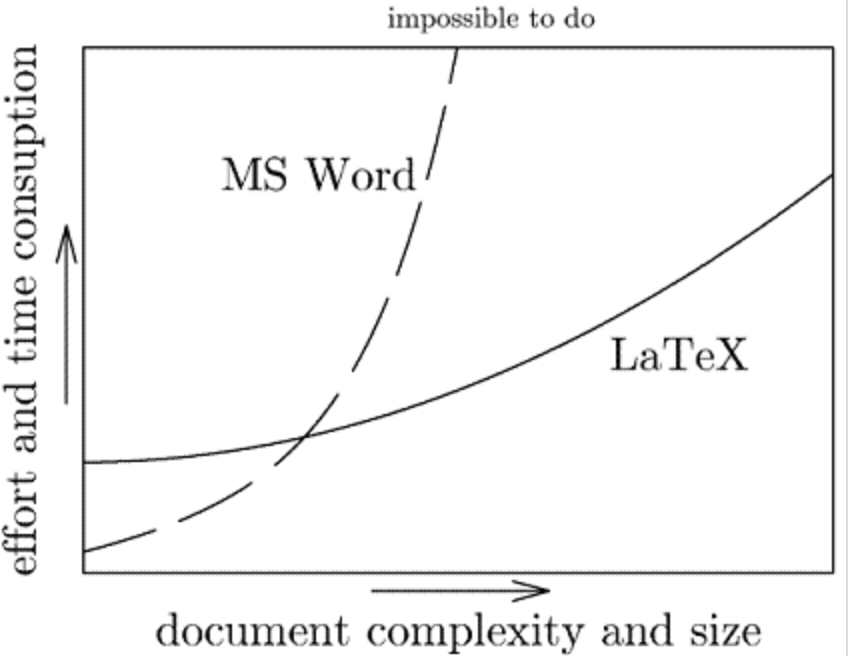
\includegraphics[width=0.75\textwidth]{latex-vs-word.png}
   \end{center}    



\end{frame}


\begin{frame}

  \frametitle{What I intend to do?}
 
  
 \begin{enumerate}
    \item Understand how the software works.
    
       \begin{itemize}
     \item The compiler
     \item The editor
     \item The final document (normally in .pdf)
      \end{itemize}
   
   \item Let you create and edit your first \LaTeX document
   
          \begin{itemize}
          \item Presentation
          \item Article
          
         
\end{itemize}
  \end{enumerate} 
 
  \end{frame}
  
  
  \begin{frame}
    \frametitle{Workflow in \LaTeX}
   

\begin{center}
\words{EDITOR} $\Rightarrow$ \words{COMPILER} $\Rightarrow$ \words{OUTPUT (.pdf)} 
\end{center}
  

 \vspace{1cm}
 
\begin{columns}
        \begin{column}{0.31\textwidth}
            
\includegraphics[width=0.95\textwidth]{latex-web.png}
        \end{column}
        
         \begin{column}{0.31\textwidth}
 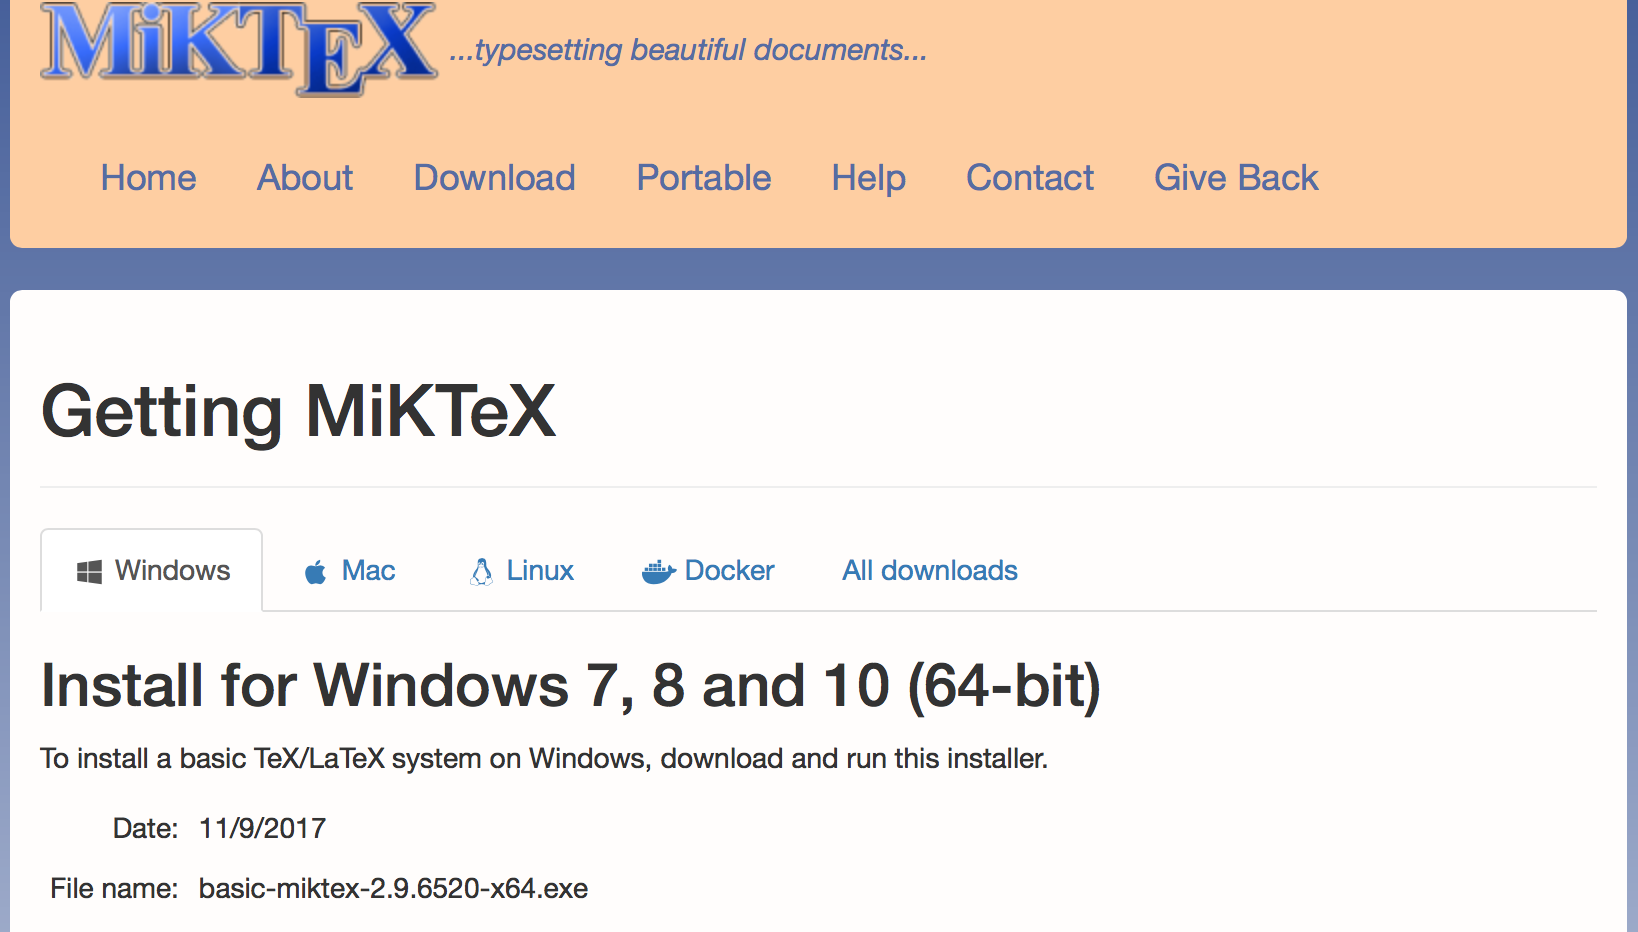
\includegraphics[width=0.95\textwidth]{miktex.png}
        \end{column}
        
         \begin{column}{0.31\textwidth}
             
\includegraphics[width=0.95\textwidth]{tex-studio.png}
        \end{column}
        
     \end{columns}
\end{frame}


 
  \end{frame}
  
\begin{frame}
               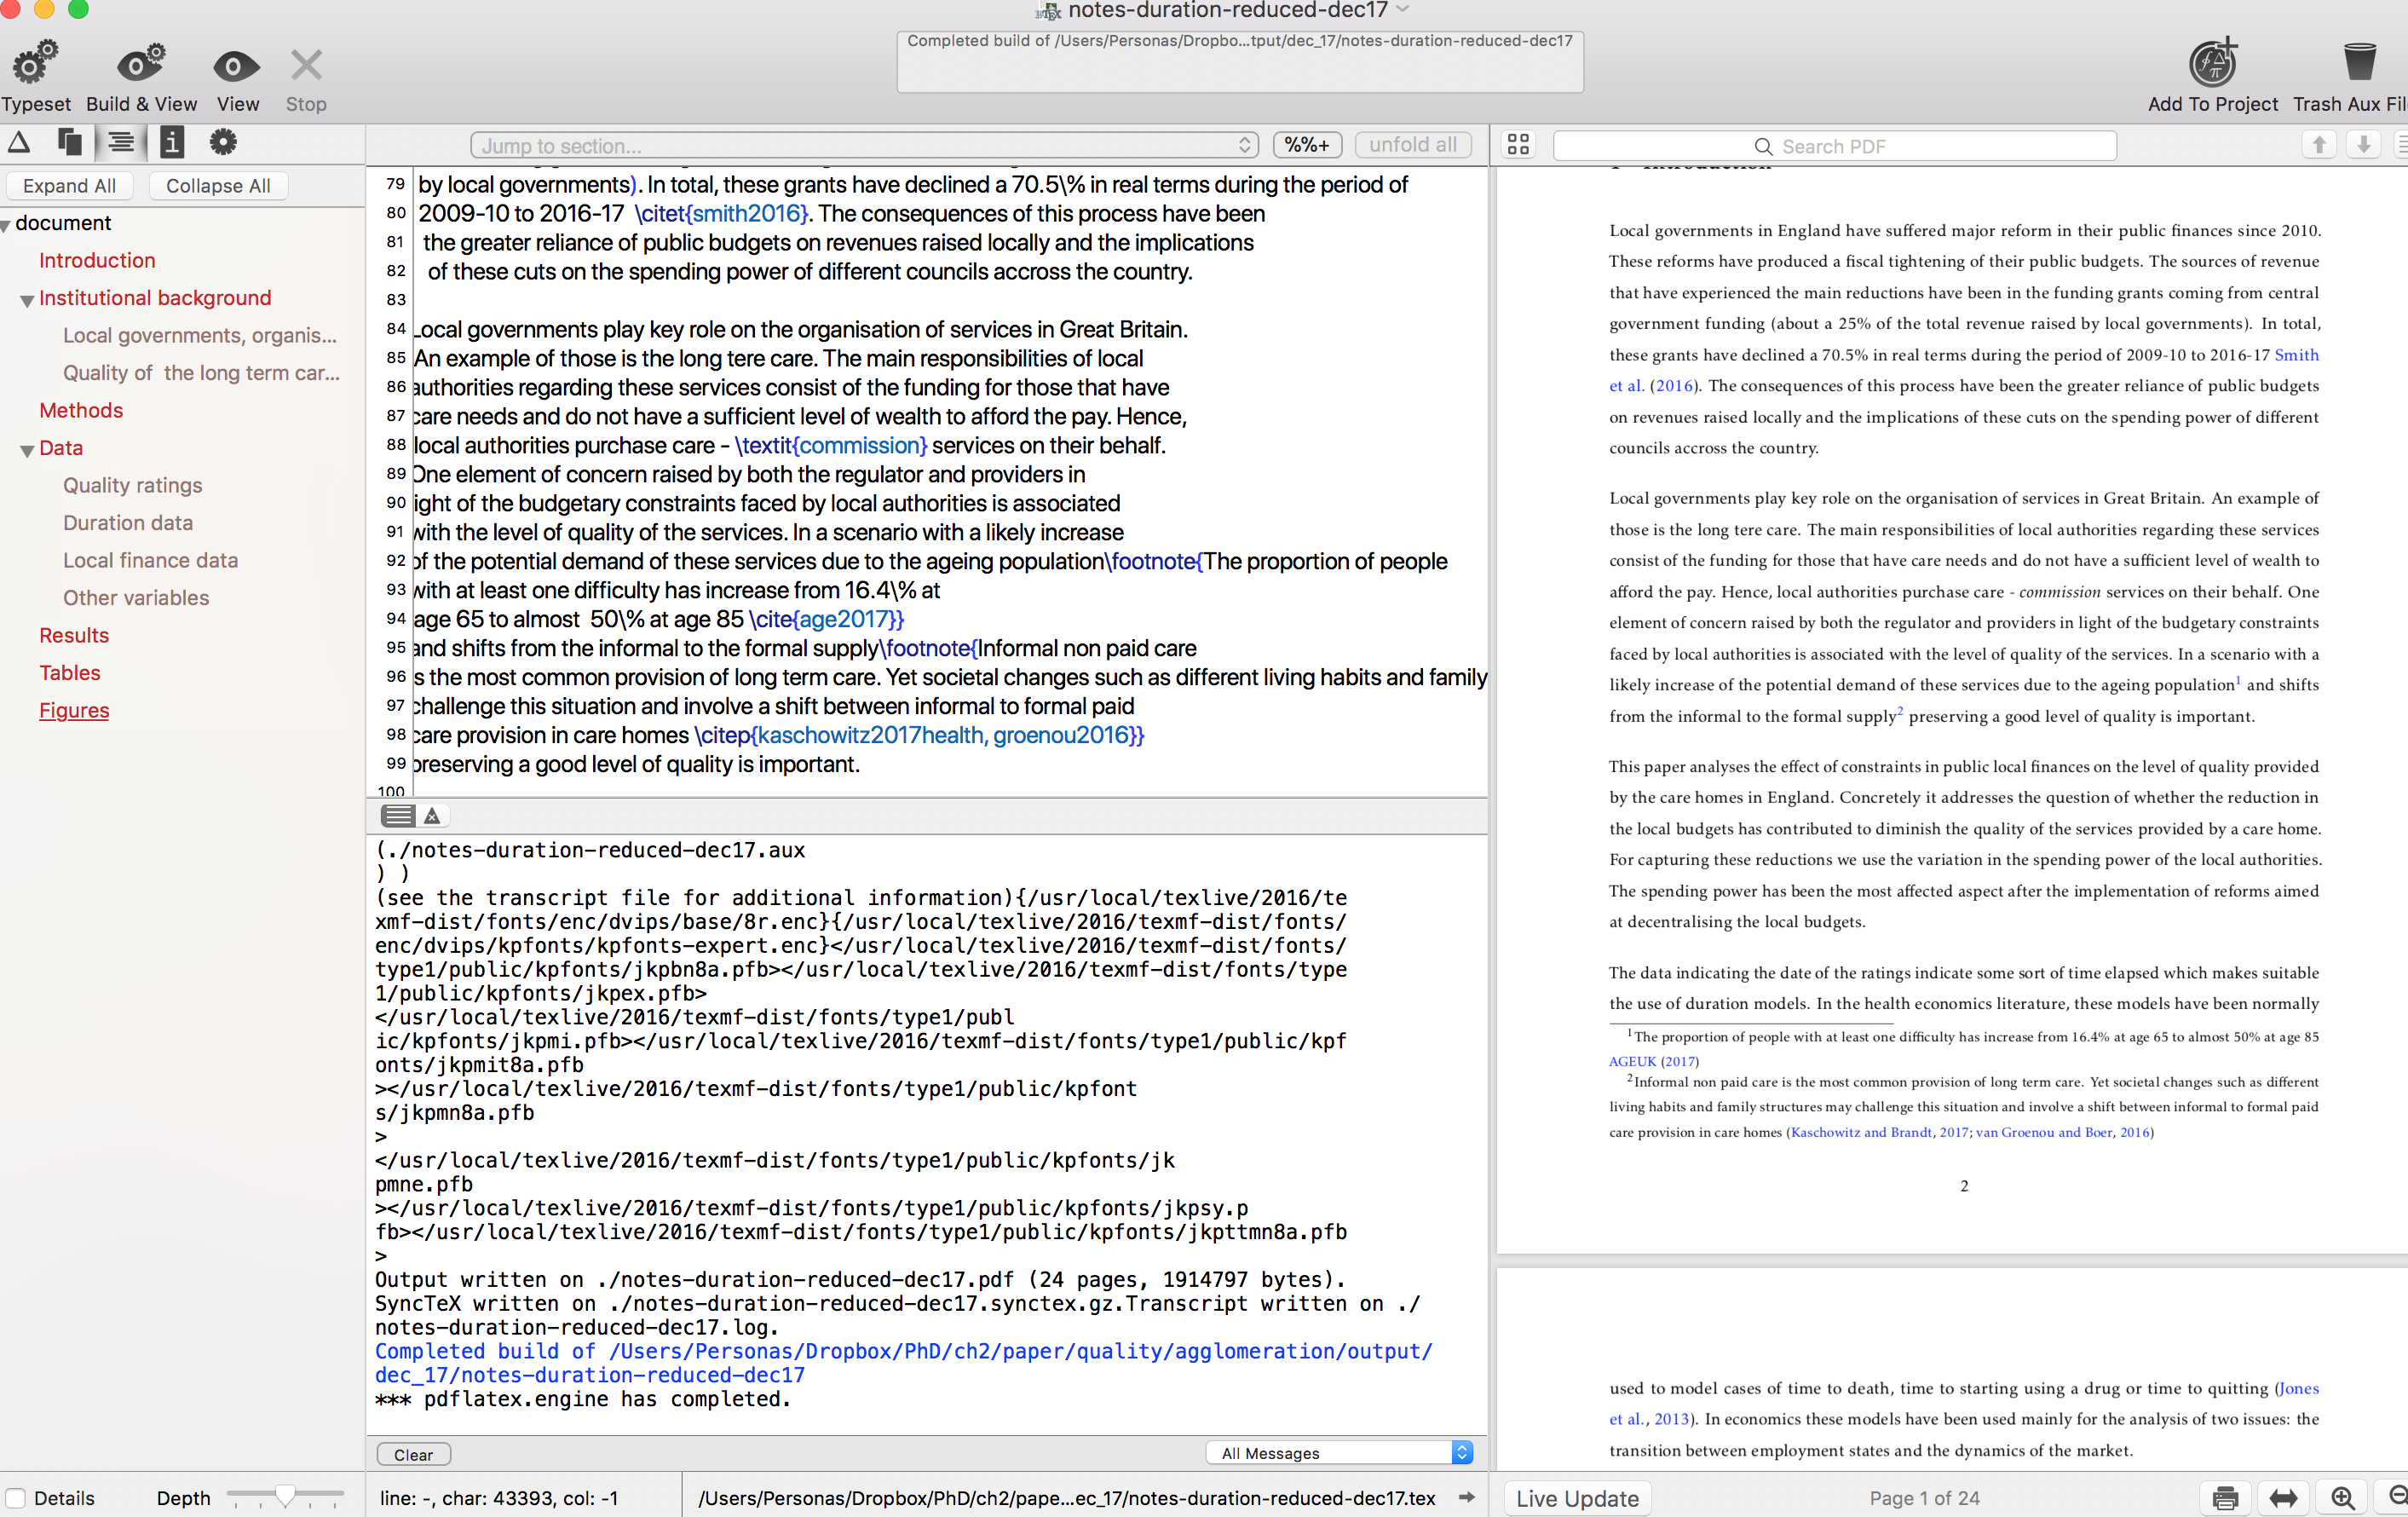
\includegraphics[width=1\textwidth]{latex-interface.png}
\end{frame}
    
  \begin{frame}
               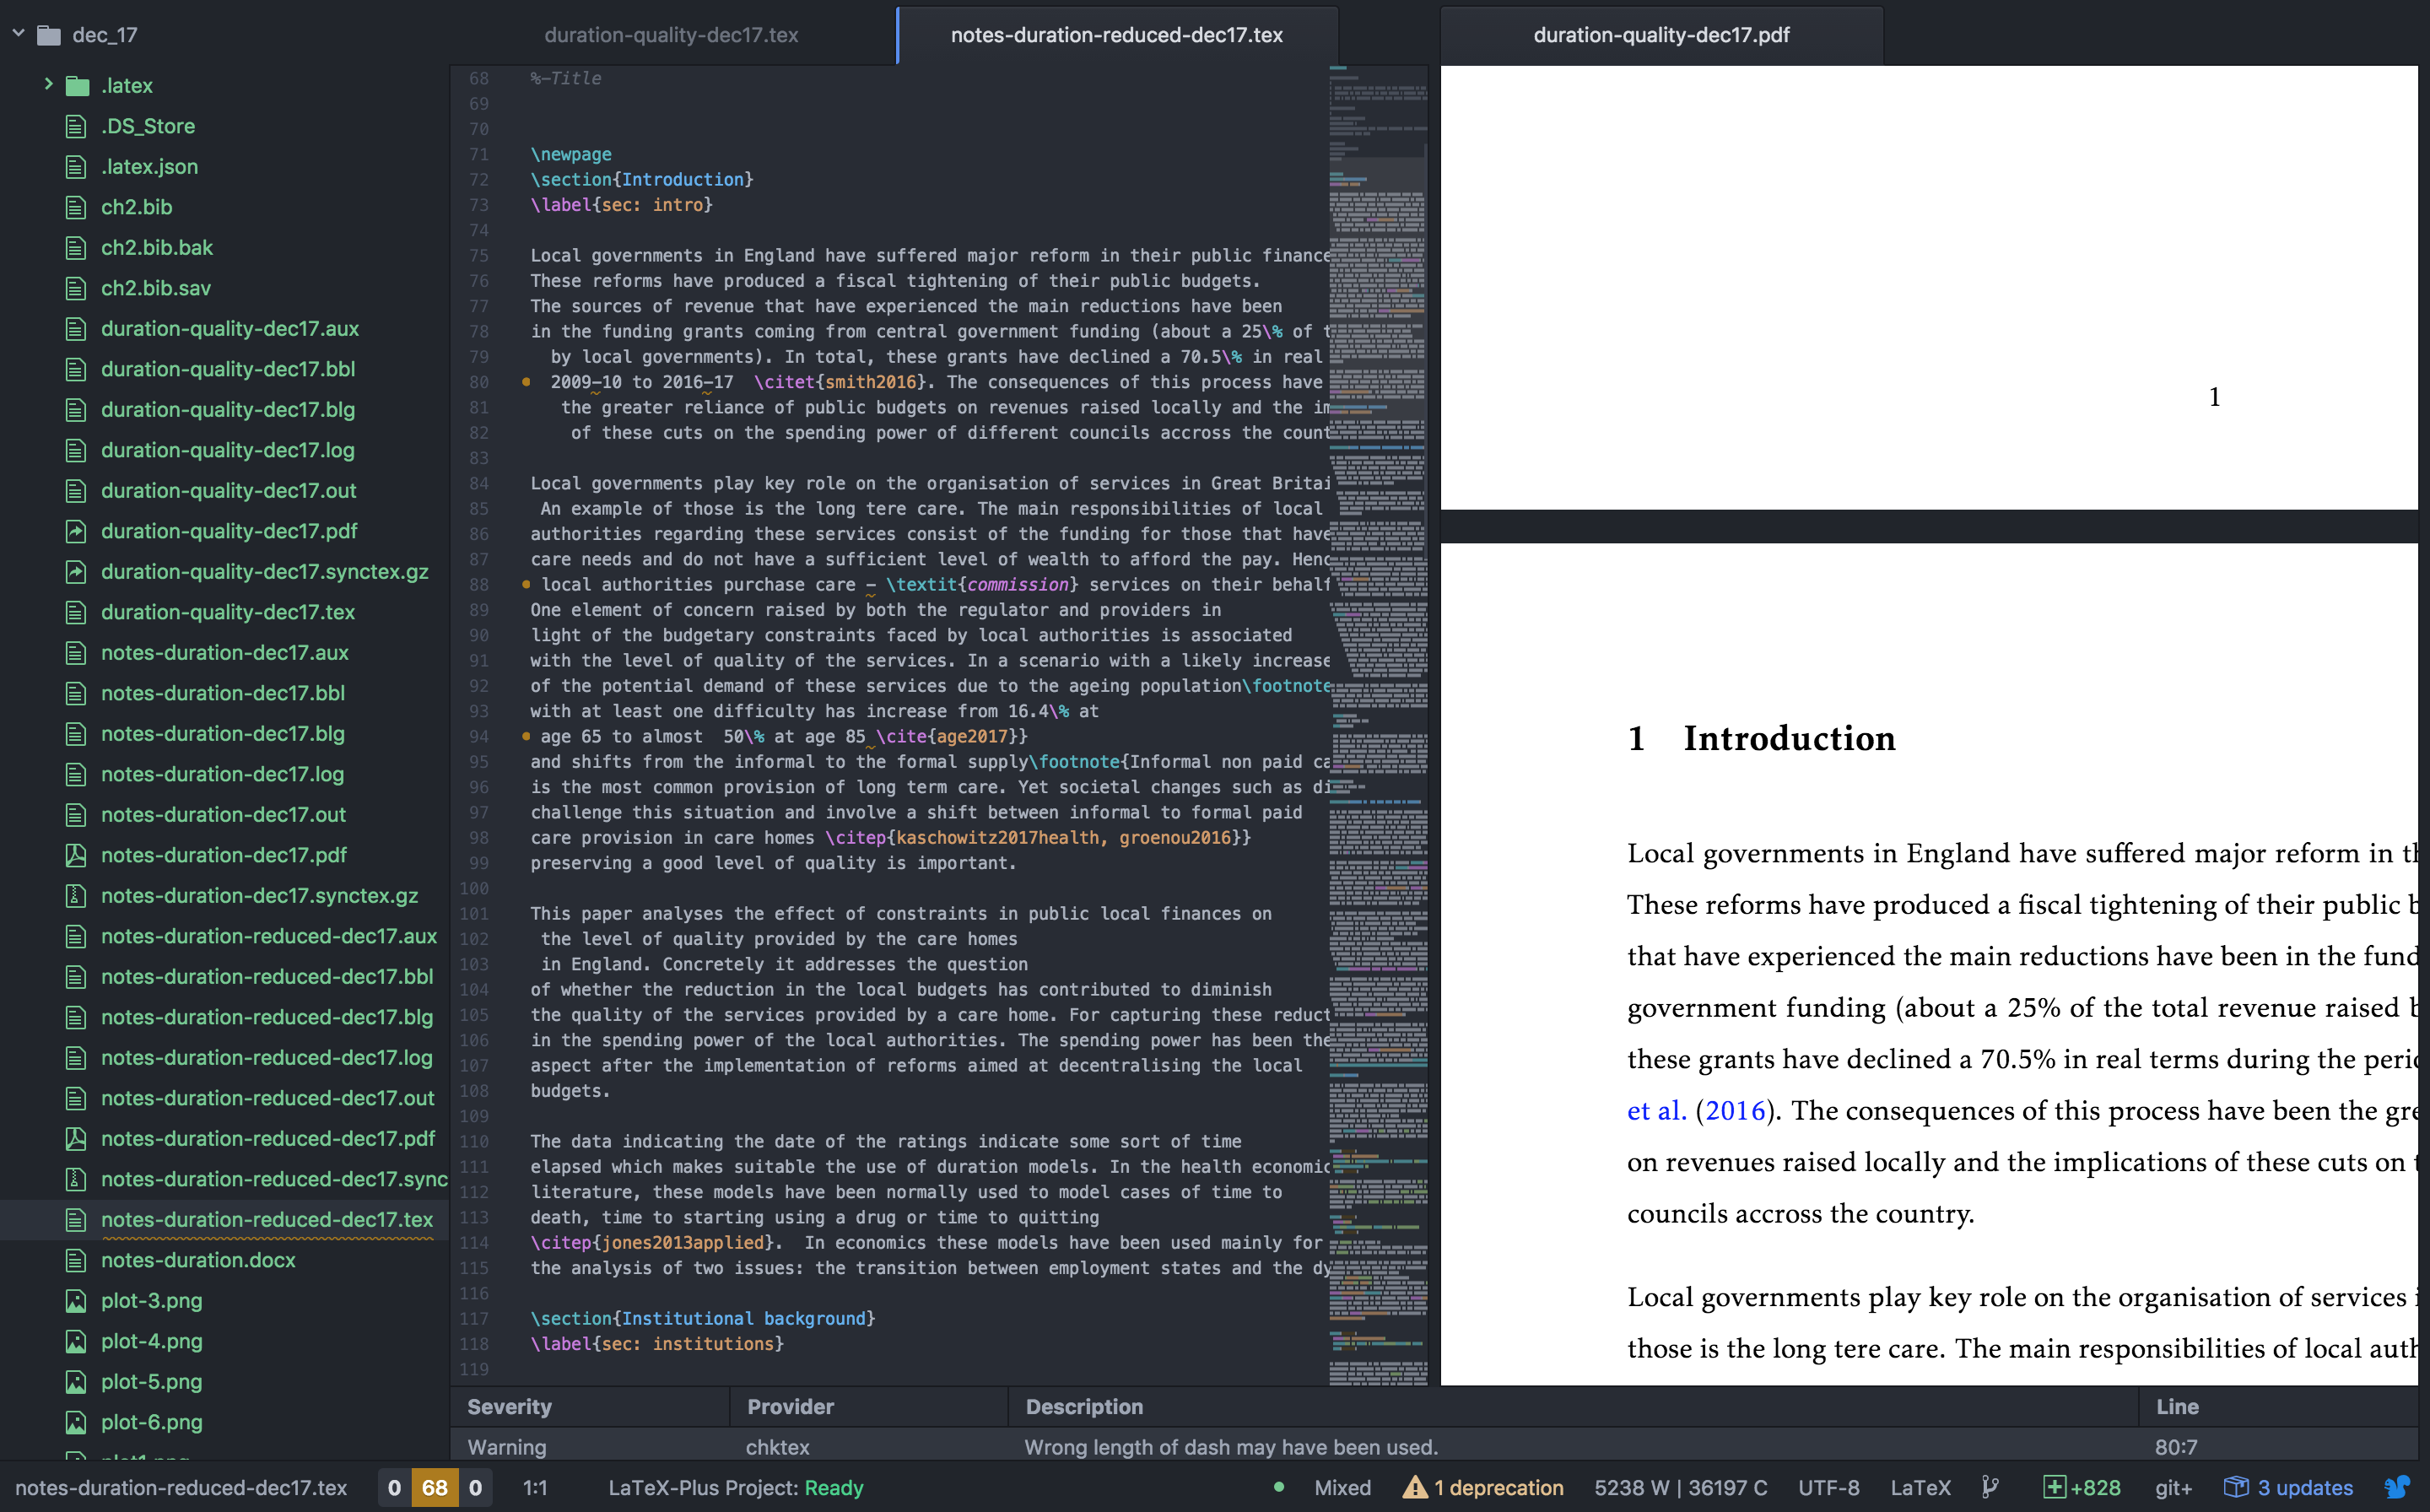
\includegraphics[width=1\textwidth]{latex-atom.png}
\end{frame}

\endgroup

    \section{Types of documents}
      \begin{frame} 
         \frametitle{The goods and bads of \LaTeX}
            
        \begin{columns}
        \begin{column}{0.4\textwidth}
                 
               \begin{center}
                 \words{\LaTeX  is good at}:
               \end{center}  
   
                   
         
      \begin{itemize}
        \item Mathematical formulas
        \item Style vs content
        \item Structure of the document
        \item Figures and tables
      \end{itemize}
      
        \end{column}
       
        
       \begin{column}{0.5\textwidth}
         
        \begin{center}
                 \words{\LaTeX  is bad  at}:
               \end{center}
               
               
                                               
      \begin{itemize}
        \item Collaboration and reproducibility
        \item Track changes and typos
        \item Count words
        \item Learning curve in the beginning
        
   
      \end{itemize}
      
         \end{column}
         
        
     \end{columns}
       
            
        \end{frame}
            
       \subsection{Presentations: the basics}

       
  
       
\begin{frame}
\frametitle{\texttt{beamer} documents}
       
          \begin{columns}
       
       
 \begin{column}{0.5\textwidth}
   \begin{itemize}
   \item The easier way to start is by using a default \texttt{beamer} template. 
   \item The  basic structure is quite similar across all \LaTeX documents. It is important 
   to specify

       \begin{enumerate}
         \item The type of document: \texttt{beamer} 
         \item The slides: \texttt{frames} 

       \end{enumerate}
  
  
  \end{itemize}    
      
 \end{column}
 
\begin{column}{0.5\textwidth}
   
   
 \begin{semiverbatim}

\code{\\documentclass\{beamer\}}

\\begin\{document\}

\code{\\begin\{frame\}}
\\frametitle\{Your title here\}
 
 Your content here....


\code{\\end\{frame\}}

\\end\{document\}
  
  


\end{semiverbatim}

 
      
  
 \end{column}
 

       \end{columns}
       \end{frame}

\begin{frame}
\frametitle{\texttt{beamer} documents: other issues in the presentation}

    
   \begin{columns}
       
       
 \begin{column}{0.5\textwidth}
   \begin{itemize}
   \item Presentations normally have a page for the title
   \item It has several components 
  

       \begin{enumerate}
         \item Title and subtitle
         \item Author
         \item Date
         \item Affiliation

       \end{enumerate}
  
  
  \end{itemize}    
      
 \end{column}
 
\begin{column}{0.6\textwidth}
   
   
 \begin{semiverbatim}
   
\\documentclass\{beamer\}

\code{ \\title\{My super presentation\}}

 \code{\\subtitle\{NERDS Group\}}
 
  \code{\\author\{Edu Gonzalo\}}
  
   \code{\\institute\{My nice department\}}
 
  \code{\\date\{15 December\}}
 
\code{\\begin\{document\}}

\\begin\{frame\}

\\frametitle\{Your title here\}
 
 Your content here....

\\end\{frame\}

\\end\{document\}
  
\end{semiverbatim}

 
      
  
 \end{column}
 

       \end{columns}


\end{frame}
 
\begin{frame}
\frametitle{\texttt{beamer} documents: other issues in the presentation}

    
   \begin{columns}
       
       
 \begin{column}{0.5\textwidth}
   \begin{itemize}
   \item Presentations normally have a page for the title
   \item It has several components 
  

       \begin{enumerate}
         \item Title and subtitle
         \item Author
         \item Date
         \item Affiliation

       \end{enumerate}
  
  \item Use \texttt{titlepage} for creating the slide with the title elements
  
  \end{itemize}    
      
 \end{column}
 
\begin{column}{0.6\textwidth}
   
   
 \begin{semiverbatim}
   
\\documentclass\{beamer\}

\code{ \\title\{My super presentation\}}

 \code{\\subtitle\{NERDS Group\}}
 
  \code{\\author\{Edu Gonzalo\}}
  
   \code{\\institute\{My nice department\}}
 
  \code{\\date\{15 December\}}
 
\code{\\begin\{document\}}

\words{\\begin\{frame\}}

\words{\\titlepage}

\words{\\end\{frame\}}

\\begin\{frame\}

\\frametitle\{Your title here\}
 
 Your content here....

\\end\{frame\}

\\end\{document\}
  
\end{semiverbatim}

 \end{column}
 

       \end{columns}


\end{frame}

\subsection{Presentations:figures}

\begin{frame}
  \frametitle{Insert figures}

  \begin{columns}
       
       
 \begin{column}{0.5\textwidth}
   \begin{itemize}
   \item Support of many formats (.png, .pdf, .jpg)
   \item Customize the location of the image on the slide
   \item Use package \texttt{graphicx}
   \item Caveats
  

       \begin{enumerate}
         
         \item Location of the images on the computer
         \item Use \texttt{figure} environment


       \end{enumerate}
       
  
  \item Use \texttt{includegraphics} for inserting the figure
  
  \end{itemize}    
      
 \end{column}
 
\begin{column}{0.6\textwidth}
   
   
 \begin{semiverbatim}
 
 \\usepackage\{graphicx\}
   
\\documentclass\{beamer\}

\\begin\{frame\}

\\frametitle\{Slide with figures\}
 
\code{\\begin\{figure\}[h]}
 
 \code{\\includegraphics[width=5cm]\{my-figure.png\}}

\code{\\end\{figure\}}

\\end\{frame\}

\\end\{document\}
  
\end{semiverbatim}

 \end{column}
 

       \end{columns}


\end{frame}

\begin{frame}
  \frametitle{Figure example}
  \begin{semiverbatim}

\\includegraphics[width=0.85\textwidth]\{merry-christmas.jpg\}
  \end{semiverbatim}
  
        
\includegraphics[width=0.85\textwidth]{merry-christmas.jpg}

\end{frame}
 
 \begin{frame}
  \frametitle{Figure example}
  
  \begin{center}
  \begin{semiverbatim}

\code{\\begin\{center\}}

\\includegraphics[width=0.85\textwidth]\{merry-christmas.jpg\}

\code{\\end\{center\}}

  \end{semiverbatim}
  \end{center}
  
  \begin{center}
        
\includegraphics[width=0.65\textwidth]{merry-christmas.jpg}
   \end{center}

\end{frame}

\begin{frame}
  \frametitle{Figure example}
  
  \begin{center}
  \begin{semiverbatim}

\\begin\{figure\}[h!]

\\centering\

\\includegraphics[width=0.85\textwidth]\{merry-christmas.jpg\}

\\caption\{I wish you merry Christmas\}

\\end\{figure\}

  \end{semiverbatim}
  \end{center}
  
  \begin{center}
    
    \begin{figure}[!h]
  \centering
 
\includegraphics[width=0.45\textwidth]{merry-christmas.jpg}
 \caption{I wish you merry Christmas}
   \end{figure}
    
       
   \end{center}

\end{frame}

\begin{frame}
  \frametitle{Columns}

  \begin{columns}
       
       
 \begin{column}{0.5\textwidth}
   \begin{itemize}



\item Sometimes you want to place your content in several columns.
\item \texttt{columns} environment.
\item Specify the width of the column

  \end{itemize}    
      
 \end{column}
 
\begin{column}{0.5\textwidth}
   
   
 \begin{semiverbatim}
 
\\begin\{frame\}

\\frametitle\{Slide with columns\}

\code{\\begin\{columns\}}

 \code{\\begin{column}\{0.5\\textwidth\}}
 
 Content column 1 ...
 
  \code{\\end{column}\{0.5\\textwidth\}}
   
  \code{\\begin{column}\{0.5\\textwidth\}}
  
  Content column 2 ...
 
  \code{\\end{column}\{0.5\\textwidth\}}

\code{\\end\{columns\}}

\\end\{frame\}


 
\end{semiverbatim}

 \end{column}
 

       \end{columns}


\end{frame}

 \subsection{Presentations:tables}

\begin{frame}
  \frametitle{Tables}

  \begin{itemize}
    \item There is not a ``one fits all'' formula
    \item Depends notably on the complexity of table 
    \item Use \texttt{table} and \texttt{tabular}
  \end{itemize}
  
  \begin{table}[!h]
\centering
\resizebox{\textwidth}{!}{%
\begin{tabular}{lcrrrrr}
  \hline
   & n & mean & sd & min & max\\
  \hline
   Positive change revenue spending power (yes = 1) & 50037 & 0.30 & 0.46 & 0.00 & 1.00 \\
   No change revenue spending power (yes = 1) & 50037 & 0.20 & 0.40 & 0.00 & 1.00 \\
  Negative change revenue spending power (yes = 1) & 50037 & 0.50 & 0.50 & 0.00 & 1.00 \\
   Population 65+ (\%) & 50037 & 0.19 & 0.05 & 0.06 & 0.34 \\
 Job seekers (\%) & 50037 & 0.01 & 0.00 & 0.00 & 0.03 \\
   Pension credit claimants (\%) & 50037 & 0.03 & 0.01 & 0.01 & 0.06 \\
  Total specific and special grants & 50037 & 226864 & 275815 & 0.00 & 1645212 \\
 District (london) (yes = 1) & 50037 & 0.10 & 0.30 & 0.00 & 1.00 \\
  \bottomrule
\end{tabular}}
\end{table}  
\end{frame}

 \begin{frame}
  \frametitle{Table: Example}
  

  \begin{semiverbatim}

\\begin\{frame\}

\\frametitle\{Table\}
 
\code{\\begin\{table\}[h]}

\code{\\centering}

\code{\\begin\{tabular\}\{lcrrrrr\}}

 \code{\\hline}
 \\ & n \& mean \& sd \& min \& max \\
  \code{\\hline}

\ Positive change ... \& 50037 \& 0.30 \& 0.46 \& 0.00 \& 1.00\\
 
   ... \& ... \& .... \& ... \& ... \& ...\

\code{\\end\{table\}}

\\end\{frame\}
  \end{semiverbatim}



\end{frame}
      
      \section{Structures}
      
      \begin{frame}
        \frametitle{Sections and subsections}
      
      \begin{itemize}
        
        \item \LaTeX keeps track of the sections (or chapters) and subsections 
        of the document
        \item It does so for every type of document you have 
        
        \begin{itemize}
          \item \texttt{section}
          \item \texttt{subsection}
        \end{itemize}
        
        \item Sections can be numbered or not  
        
            \begin{itemize}
          \item \texttt{section\{Introduction\}}
          \item \texttt{subsection*\{hypotesis\}}
        \end{itemize}
        
        
      \end{itemize}
      
      
      \end{frame}
      
\end{document}